\chapter{Проектирование и реализация ПО}

\begin{figure}[H]
	\begin{center}
		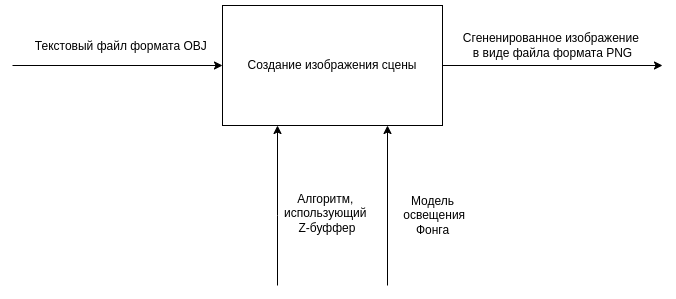
\includegraphics[width=\linewidth]{images/idf0}
	\end{center}
	\captionsetup{justification=centering}
	\caption{IDEF0 диаграмма работы программы}
	\label{img:s1}
\end{figure}

\section{Формат входных и выходных данных и обоснование выбора}
Для представления входных данных был выбран текстовый файл формата OBJ -- формат описания геометрии.

Преимущества формата:
\begin{itemize}
	\item открытый формат файла, что позволяет его редактировать, в отличие от бинарных форматов;
	\item занимает первое место по количеству моделей в рейтинге, указанным в статье \cite{bib8};
	\item не привязан к определенной программе, поэтому может быть экспортирован/импортирован во многие программы. 
\end{itemize}
""\newline
""\newline
\begin{lstlisting}[caption={Пример .obj файла}]
# comment
o figure

v 10 20 30 
v 40 50 100
v -10 20 40

f 1 2 3

Ka 255 200 180	
\end{lstlisting}

\begin{itemize}
	\item \# -- комментарий
	\item o -- название фигуры
	\item v -- параметры вершины
	\item f -- определение поверхности 
	\item Ka -- внешний цвет поверхности(RGB)
\end{itemize}

Также в файле могут быть заданы vn(нормали), vt(текстуры вершины), g(группировка объектов), usemtl(параметры материала, цветовых характеристик и прозрачности).
\newline

Из всех возможных форматов изображений для выходных данных (BMP, GIF, JPG, JPEG, PNG, PBM, PGM, PPM, XBM, XPM), которая предоставляет библиотека Qt, был выбран формат PNG, так как:
\begin{itemize}
\item формат PNG -- графический, что необходимо для создания фильма с помощью утилиты FFmpeg [6];
\item формат PNG является платформонезависимым, в отличие от формата BMP;
\item изображения в формате PNG более качественные, чем изображения в формате JPG по метрике типа PSN \cite{bib9}.
\end{itemize}

\section{Реализуемые алгоритмы}

\subsection{Алгоритм, использующий Z-буфер}
Данный алгоритм работает в пространстве изображения \cite{bib10}. Используется два буфера:
\begin{itemize}
	\item буфер кадра, в котором хранятся атрибуты каждого пикселя в про-
	странстве изображения;
	\item z-буфер, куда помещается информация о координате z для каждого
	пикселя.
\end{itemize}

Первоначально в z-буфере находятся минимально возможные значения z, а в буфере кадра располагаются пиксели, описывающие фон. Каждый многоугольник преобразуется в растровую форму и записывается в буфер кадра. В процессе подсчета глубины нового пикселя, он сравнивается с тем значением, которое уже лежит в z-буфере. Если новый пиксель расположен ближе к наблюдателю, чем предыдущий, то он заносится в буфер кадра и происходит корректировка z-буфера.

Для решения задачи вычисления глубины z каждый многоугольник описывается уравнением $ax + by + zc + d = 0$. При c = 0 многоугольник для наблюдателя вырождается в линию.

В программе была использованна модификация указанного алгоритма путем добавления вычисления теневого z-буфера из точки наблюдения, совпадающей с источником света.

На рисунке 2.2 изображена схема модифицированного алгоритма z-буфера.
\begin{figure}[H]
	\begin{center}
		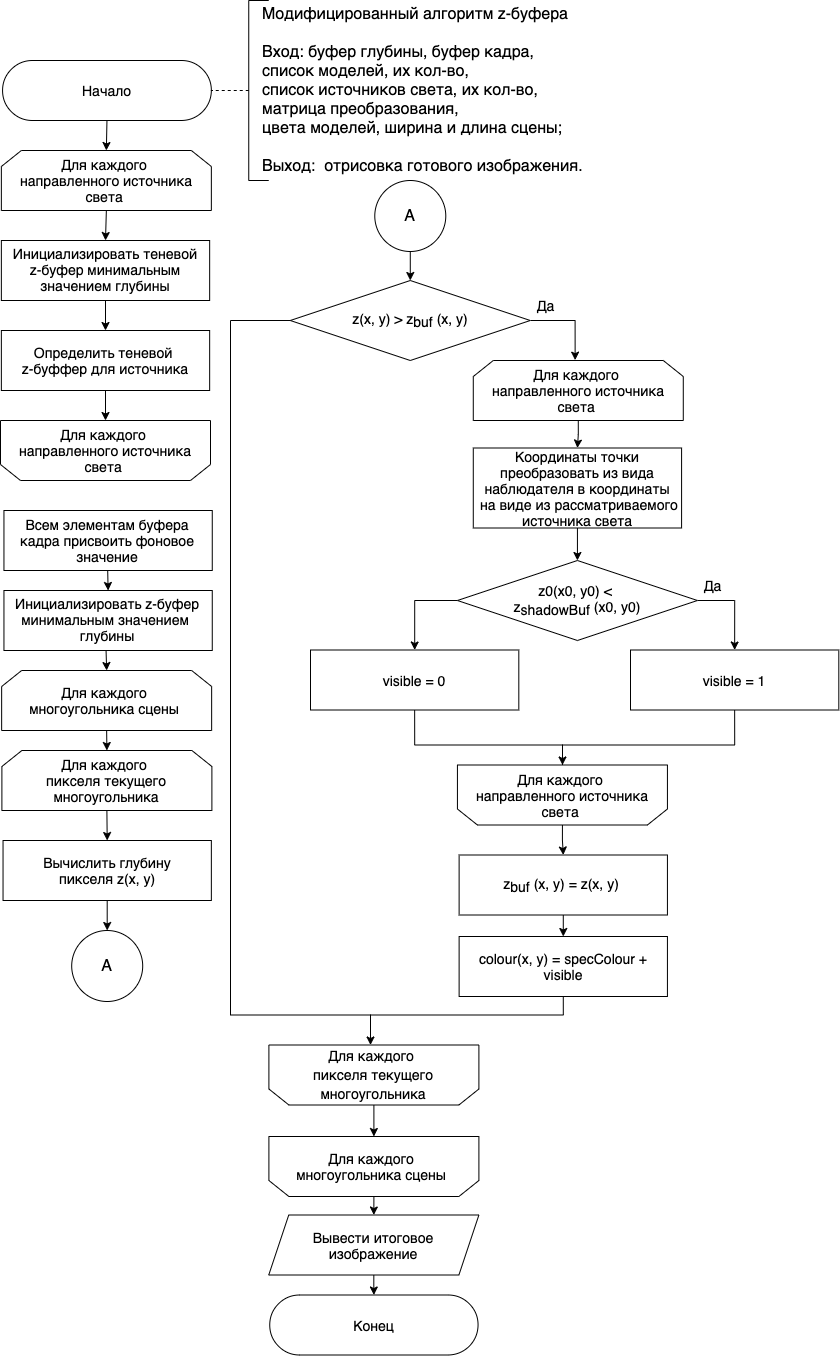
\includegraphics[scale=0.45]{images/alg}
	\end{center}
	\captionsetup{justification=centering}
	\caption{модифицированный алгоритма z-буфера}
	\label{img:s1}
\end{figure}


\subsection{Модель освещения Фонга}
Модель Фонга -- классическая модель освещения \cite{bib11}. Пусть заданы точечный источник света, расположенный в некоторой точке, поверхность, которая будет освещаться и наблюдатель. Каждая точка поверхности имеет свои координаты и в ней определена нормаль к поверхности. Её освещенность складывается из трех компонент:
\begin{itemize}
	\item фоновое освещение (ambient);
	\item рассеянный свет (diffuse);
	\item бликовая составляющая (specular). 
\end{itemize}

Фоновое освещение это постоянная в каждой точке величина надбавки к освещению. Вычисляется фоновая составляющая освещения по формуле 2.1:

\begin{equation}
I_a = k_a i_a
\end{equation}

$I_a$ - фоновая составляющая освещенности в точке

$k_a$ – свойство материала воспринимать фоновое освещение

$I_a$ – мощность фонового освещения
\newline

Рассеянный свет при попадании на поверхность рассеивается равномерно во все стороны. При расчете такого освещения учитывается только нормаль к поверхности и направление на источник света. Рассеянная составляющая рассчитывается по закону косинусов (закон Ламберта):

\begin{equation}
I_d=k_d {\cos{(\vec{L},\vec{N})}}i_d=k_d(\vec{L}\cdot\vec{N})i_d, где
\end{equation}

$I_d$ – рассеянная составляющая освещенности в точке

$k_d$ – свойство материала воспринимать рассеянное освещение

$i_d$ – мощность рассеянного освещения

$\vec{L}$ – направление из точки на источник

$\vec{N}$ - вектор нормали в точке.
\newline

Зеркальный свет при попадании на поверхность подчиняется следующему закону: <<Падающий и отраженный лучи лежат в одной плоскости с нормалью к отражающей поверхности в точке падения, и эта нормаль делит угол между лучами на две равные части>>. То есть отраженная составляющая освещенности в точке зависит от того, насколько близки направления на наблюдателя и отраженного луча. Это можно выразить формулой 2.3:

\begin{equation}
	I_s=k_s {\cos^{\alpha}{(\vec{R},\vec{V})}}i_s=k_s(\vec{R}\cdot\vec{V})^{\alpha}i_s , где
\end{equation}

$I_s$ – зеркальная составляющая освещенности в точке,

$k_s$ – коэффициент зеркального отражения,

$i_d$ – мощность зеркального освещения,

$\vec{R}$ – направление отраженного луча,

$\vec{V}$ - направление на наблюдателя,

$\alpha$ - коэффициент блеска, свойство материала.
\newline

Тогда интенсивность света подсчитывается формулой 2.4:

\begin{equation}
	I_s= I_a + I_d + I_s = k_a i_a + k_d(\vec{L}\cdot\vec{N})i_d + k_s(\vec{R}\cdot\vec{V})^{\alpha}i_s
\end{equation}

Пример работы модели Фонга:

\begin{figure}[H]
	\begin{center}
		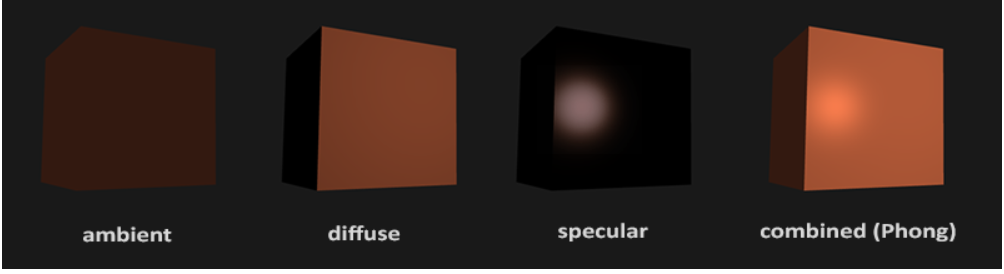
\includegraphics[width=\linewidth]{images/phong}
	\end{center}
	\captionsetup{justification=centering}
	\caption{Модель освещения Фонга}
	\label{img:s1}
\end{figure}

\section{Сценарий Gitlab CI/CD}

\begin{figure}[H]
	\begin{center}
		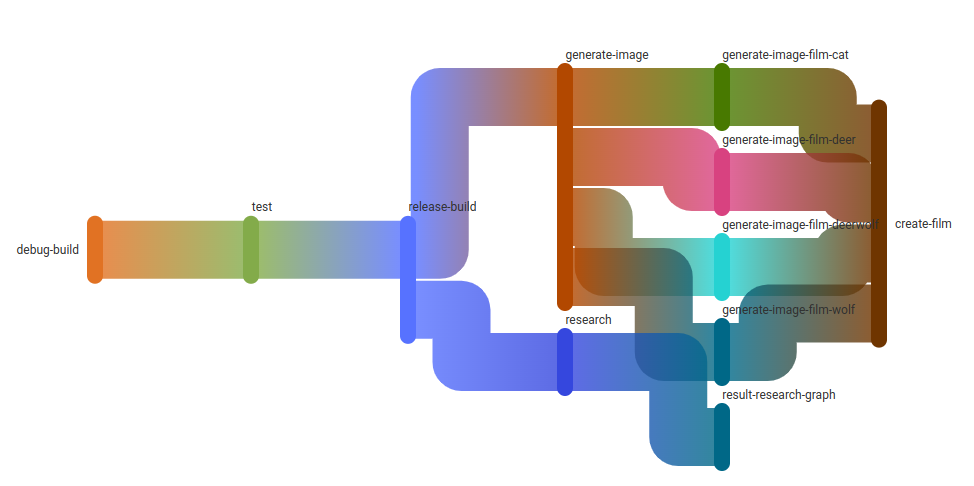
\includegraphics[width=\linewidth]{images/gitlab}
	\end{center}
	\captionsetup{justification=centering}
	\caption{Сценарий Gitlab CI/CD}
	\label{img:s1}
\end{figure}


Сценарий состоит из семи стадий:
\begin{itemize}
	\item build\_debug -- сборка отладочной версии программы.
		\begin{itemize}
			\item debug-build -- задание команд для сборки отладочной версии программы.
		\end{itemize}
	\item testing -- модульное тестирование программы.
		\begin{itemize}
			\item unit-test -- модульное тестирование.
		\end{itemize}
	\item build\_release -- сборка версии программы на выпуск.
		\begin{itemize}
			\item release-build-- задание команд для сборки версии программы на выпуск
		\end{itemize}
	\item generate\_image -- получение изображения сцены.
		\begin{itemize}
			\item generate-image -- получение изображении указанной сцены.
		\end{itemize}
	\item generate\_image\_film -- генерация нескольких изображений изменяемой сцены.
		\begin{itemize}
			\item generate-image-film-deer
			\item generate-image-film-catwolf
			\item generate-image-film-trees
		\end{itemize}
	\item create\_film -- создание фильма из полученных изображений сцен на предыдущей стадии.
		\begin{itemize}
			\item create-film -- задание команд для создания фильма на основе изображений из прошлой стадии.
		\end{itemize}
	\item research -- исследование временных характеристик программы.
		\begin{itemize}
			\item research -- замер времени работы программы при разном количестве полигонов на сцене.
			\item result-research-graph -- преобразование данных и построение графика зависимости времени работы программы от количества полигонов на сцене.
		\end{itemize}
\end{itemize}


\lstinputlisting[caption={.gitlab-ci.yml файл}]{code/.gitlab-ci.yml}
\newpage
\section{Docker}
Для различных заданий сценария Gitlab CI/CD были использованы
различные образы Docker с DockerHub \cite{bib3}:
\begin{itemize}
	\item darkmattercoder/qt-build:latest 
	
	Окружение сборки и запуска приложения QT. Тег latest предоставляет последнюю выпущенную qt версию для среды сборки. 
	
	Стадии, использующие этот образ: все задания стадии build\_debug, testing, build\_release, generate\_image, generate\_image\_film, \\задание research-time стадии research
	
	Зависимости этого образа:
	\begin{itemize}
		\item ca-certificates;
		\item sudo (для возможности изменять контейнер от имени администратора);
		\item curl;
		\item python
		\item gperf;
		\item bison;
		\item flex;
		\item build-essential;
		\item pkg-config;
		\item libgl1-mesa-dev;
		\item libicu-dev;
		\item firebird-dev;
		\item libmysqlclient-dev;
		\item libpq-dev;
		\item bc;
		\item git;
		\item зависимости xcb;
		\item bash;
		\item libdbus-1-dev (для Qt версии 5.14.0 и выше);
		\item libnss3-dev (для Qt версии 5.14.0 и выше).
	\end{itemize}
	\item jrottenberg/ffmpeg
	
	Мнималистичный контейнер Docker с утилитой FFmpeg, которая компилируется из файлов исходного кода. 
	
	Стадии, использующие этот образ: create\_film.
	
	Зависимости этого образа:
	\begin{itemize}
		\item automake;
		\item bzip2;
		\item cmake;
		\item diffutils;
		\item expat-devel;
		\item gcc;
		\item git;
		\item gperf;
		\item libtool;
		\item make;
		\item nasm;
		\item perl;
		\item python3;
		\item openssl-devel;
		\item tar;
		\item yasm;
		\item which;
		\item zlib-devel.
	\end{itemize}
	
	\item python
	
	Официальный образ Docker, поддерживаемый одноименным сообществом. Содержит только минимальное количество пакетов, необходимых для запуска python.
	
	Стадии, использующие этот образ: задание result-research-graph стадии research.
	
	Зависимости этого образа:
	\begin{itemize}
		\item dpkg-dev;
		\item gcc;
		\item gnupg dirmngr;
		\item libbluetooth-dev;
		\item libbz2-dev;
		\item libc6-dev;
		\item libexpat1-dev; 
		\item libffi-dev;
		\item libgdbm-dev; 
		\item liblzma-dev;
		\item libncursesw5-dev;
		\item libreadline-dev; 
		\item libsqlite3-dev; 
		\item libssl-dev;
		\item make;
		\item tk-dev;
		\item uuid-dev; 
		\item wget;
		\item xz-utils;
		\item zlib1g-dev.
	\end{itemize}
\end{itemize}

\section{Модульное тестирование}

Для модульного тестирования был использован фреймворк QT Test, описанный в пункте 1.4.

Чтобы создать тест, необходимо создать подкласс QObject с названием Test\$, где \$- имя тестируемого класса. 


\lstinputlisting[caption={Создание класса TestTriangle}]{code/test.h}

В приватных слотах класса создаются тесты, которые используют макросы фреймворка QT Test.

\lstinputlisting[caption={Модулный тест}]{code/test.cpp}

Чтобы добавить модульный тест, необходимо создать ещё один приватный слот в классе Test\$.

\newpage
\section{Управление из командной строки}

Для автоматизации процессов в программе реализовано управление из командной строки:
\begin{itemize}
	\item ключ <<-scene>>, после которого идет название OBJ файла, используется для загрузки сцены из указанного файла;
	\item ключ <<-image>>, после которого идет название PNG файла, используется для генерации изображения и сохранение его в файл с указанным названием;
	\item ключ <<-film>> используется для генерации PNG изображений поворота сцены для фильма;
	\item ключ <<-research>> используется для замера времени отрисовки сцены;
	\item ключ <<-test>> используется для модульного тестирования.
\end{itemize}


\section{Пример работы программы}
\begin{figure}[H]
	\begin{center}
		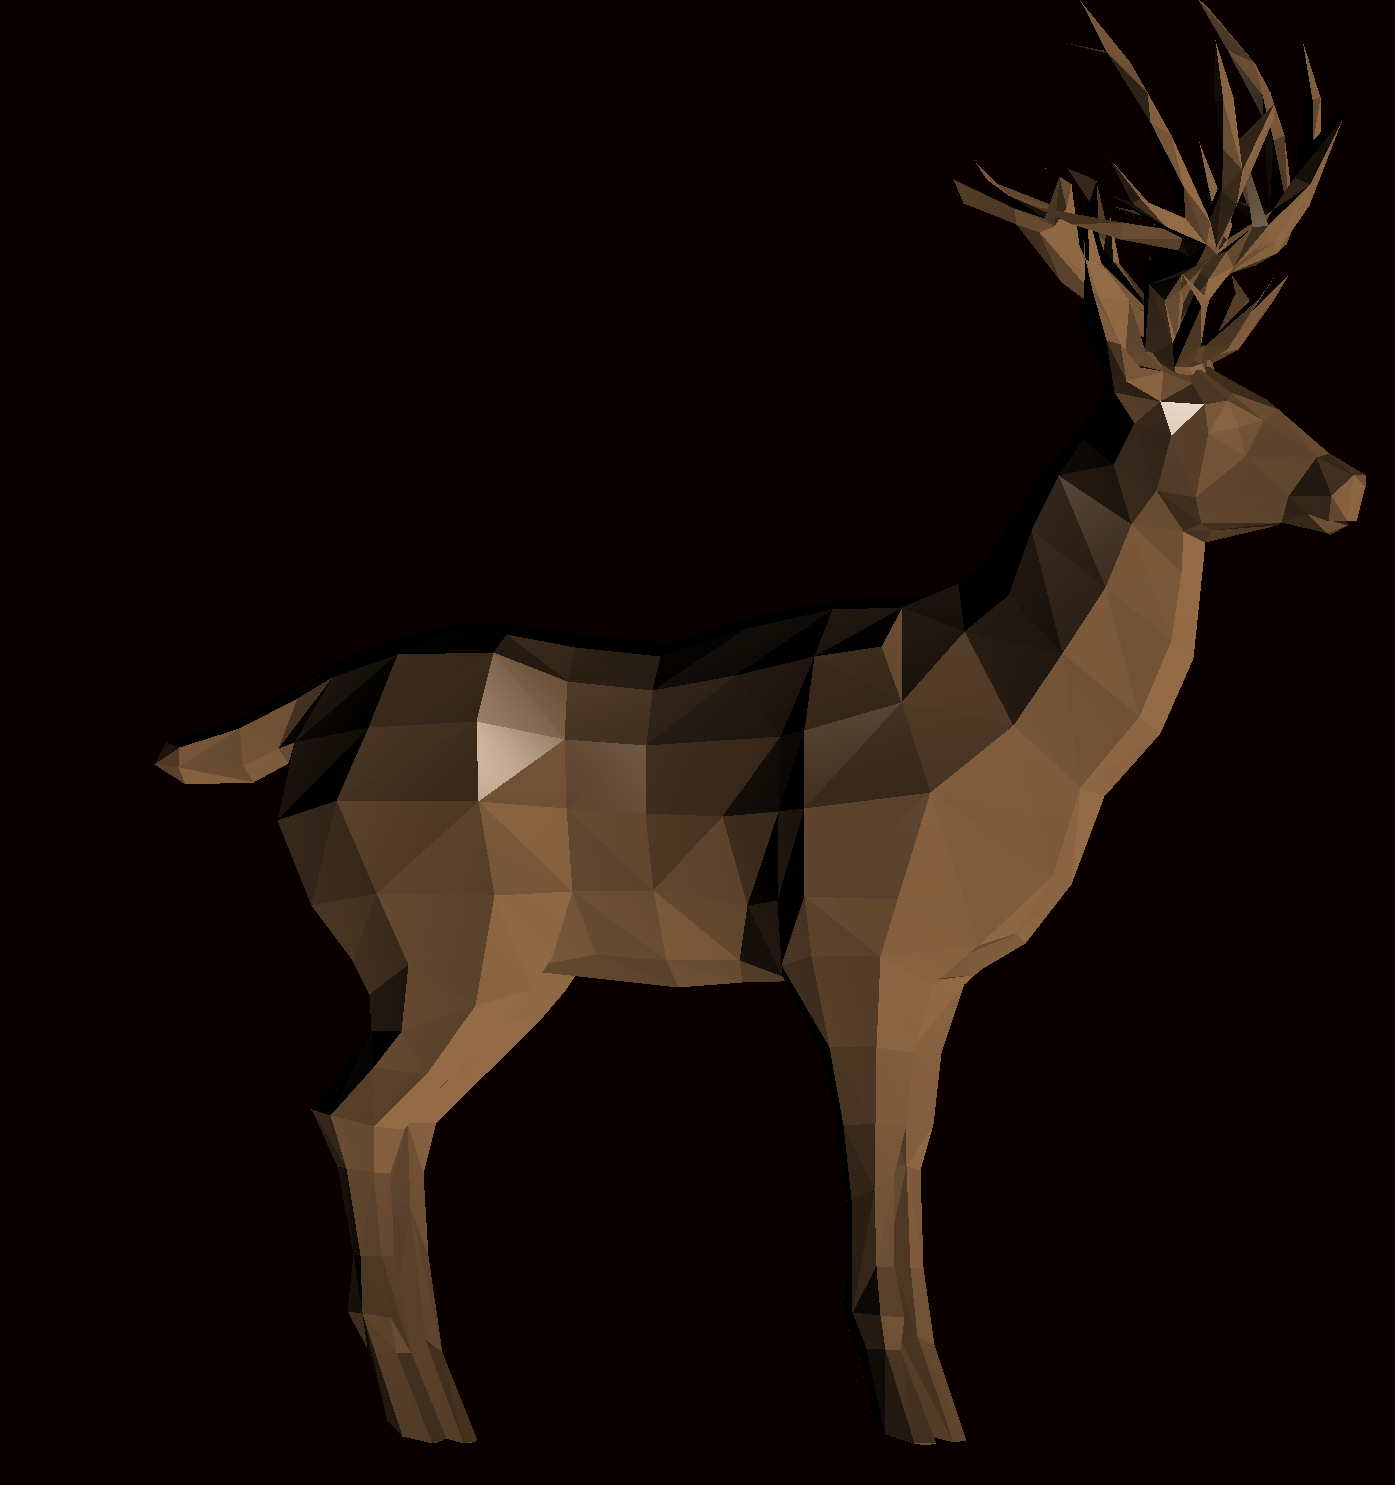
\includegraphics[scale=0.33]{images/deer}
	\end{center}
	\captionsetup{justification=centering}
	\caption{Олень. 1508 полигонов}
	\label{img:s1}	
\end{figure}

\begin{figure}[H]
	\begin{center}
		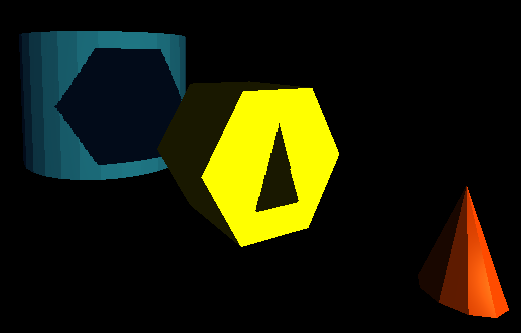
\includegraphics[scale=0.5]{images/shadow}
	\end{center}
	\captionsetup{justification=centering}
	\caption{Сцена с тенями. 300 полигонов}
	\label{img:s1}	
\end{figure}


\begin{figure}[H]
	\begin{center}
		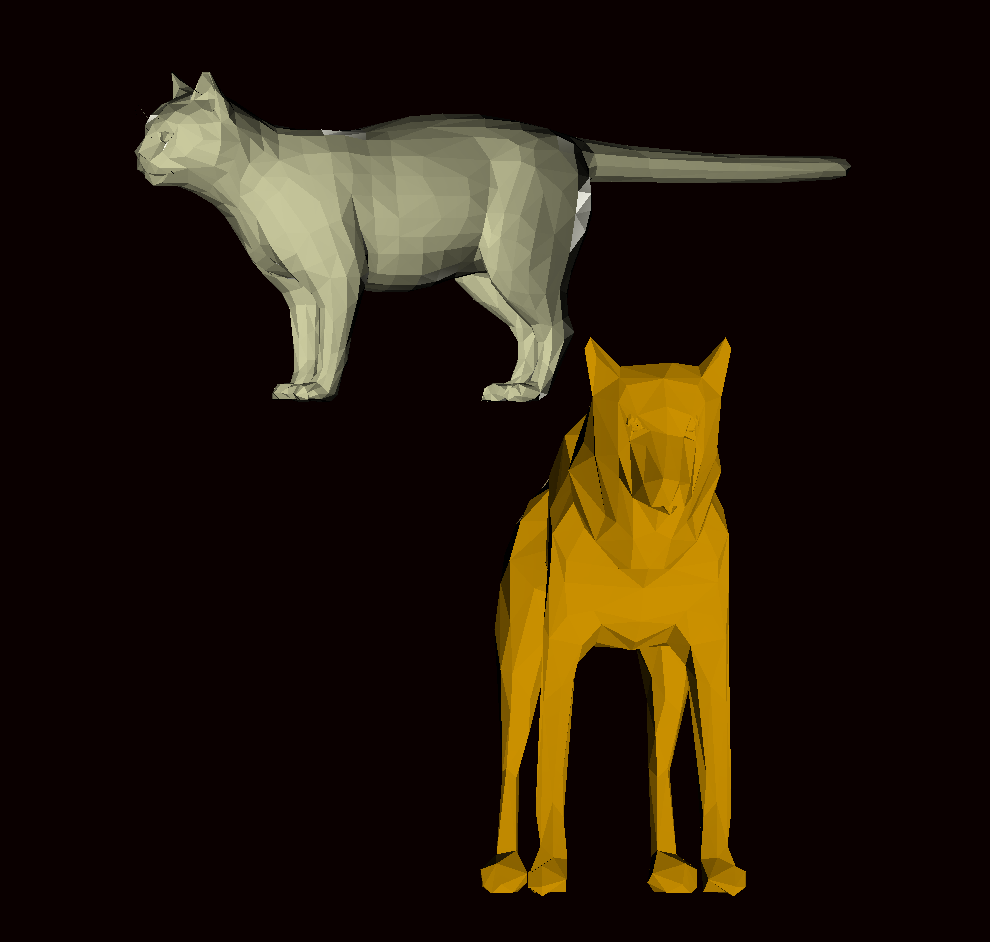
\includegraphics[scale=0.45]{images/catwolf}
	\end{center}
	\captionsetup{justification=centering}
	\caption{Кот и волк. 3038 полигонов}
	\label{img:s1}
\end{figure}

\begin{figure}[H]
	\begin{center}
		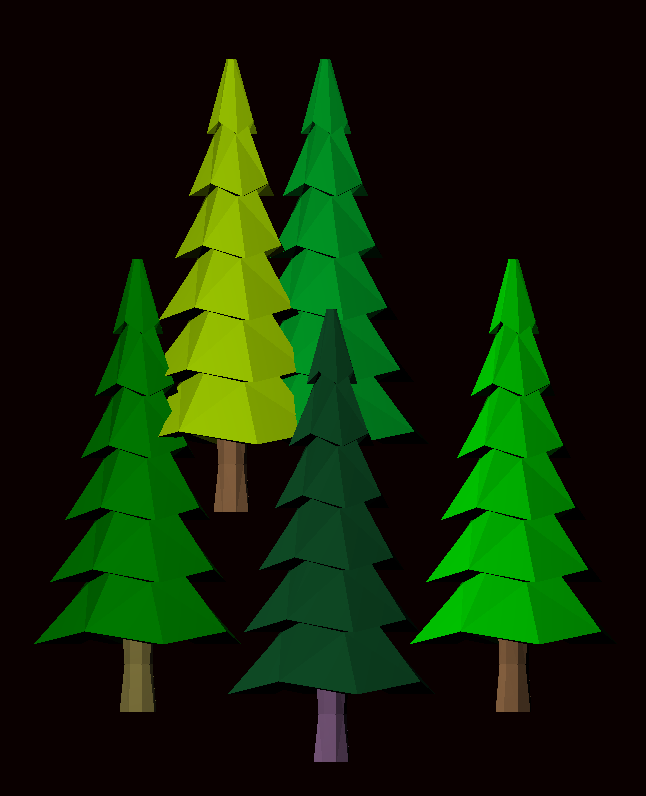
\includegraphics[scale=0.5]{images/tree}
	\end{center}
	\captionsetup{justification=centering}
	\caption{Деревья. 1240 полигонов}
	\label{img:s1}
\end{figure}

Было проведено исследование временных характеристик программы от числа полигонов на сцене. Из полученных данных был построен график, изображенный на рисунке 2.9:
\begin{figure}[H]
	\begin{center}
		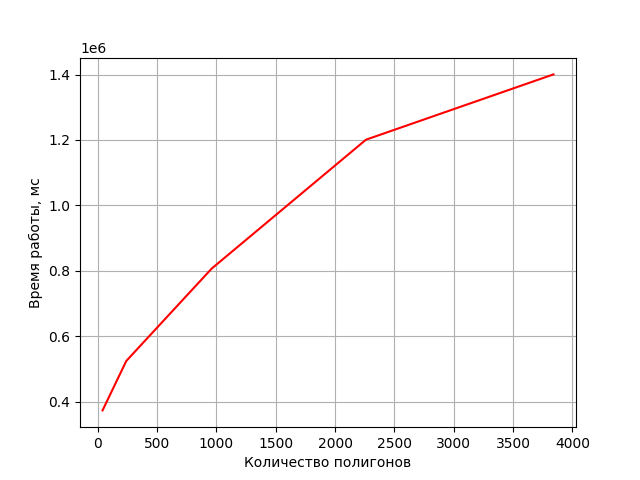
\includegraphics[scale=1]{images/result}
	\end{center}
	\captionsetup{justification=centering}
	\caption{Зависимость времени работы программы от количества полигонов}
	\label{img:s1}
\end{figure}
По итогам исследования можно сказать, что время работы алгоритма линейно увеличивается при увеличении числа полигонов на сцене.